\documentclass[crop,tikz]{standalone}

\tikzset{>=latex}
\newcommand{\place}{\vec{r}}
\newcommand{\F}{\vec{F}}

\begin{document}
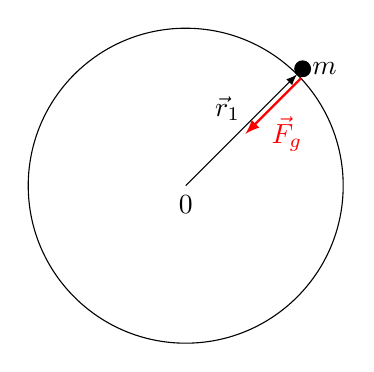
\begin{tikzpicture}
  \draw[] (0,0) circle (2);
  \draw[fill,black] (45:2.1) circle (0.1) node[right] {$m$};
  \draw[->] (0,0) -- node[above,xshift=-0.5em] {$\place_1$} (45:2);
  \node[below] at (0,0) {$0$};
  \begin{scope}[shift={(0.05,-0.05)}]
    \draw[->,red,thick] (45:2) -- node[below,xshift=0.5em] {$\F_g$} (45:1);
  \end{scope}
\end{tikzpicture}
\end{document}
